\documentclass[crop=false,a4paper,oneside,11pt]{standalone}
\usepackage{a4wide,graphicx,fancyhdr,amsmath,amssymb,float,graphicx,color,geometry,xcolor,titlesec,colortbl,tabu}
\usepackage[parfill]{parskip}
\usepackage[nodayofweek]{datetime}
%----------------------- Macros and Definitions --------------------------

%fast change of things
\newcommand{\mysubject}{2IO70 DBL Embedded Systems}
\newcommand{\myassignment}{Group 12}

%\definecolor{titlepagecolor}{cmyk}{1,.60,0,.40}
%\definecolor{namecolor}{cmyk}{1,.50,0,.10}


\setlength\headheight{20pt}
\addtolength\topmargin{-10pt}
\addtolength\footskip{20pt}

% Define light and dark Microsoft blue colours
\definecolor{MSBlue}{rgb}{.204,.353,.541}
\definecolor{MSLightBlue}{rgb}{.31,.506,.741}
\arrayrulecolor{MSLightBlue}

% Set formats for each heading level

\titleformat*{\section}{\Large\bfseries\sffamily\color{MSBlue}}
\titleformat*{\subsection}{\large\bfseries\sffamily\color{MSLightBlue}}

%date format
\newdateformat{mydate}{\monthname[\THEMONTH] \THEYEAR}

\fancypagestyle{plain}{%
\fancyhf{}
\renewcommand{\headrulewidth}{0pt}
\renewcommand{\footrulewidth}{0pt}
}

\pagestyle{fancy}
\fancyhf{}
\fancyfoot[CO] {\thepage}
\renewcommand{\headrulewidth}{0pt}
\renewcommand{\footrulewidth}{0pt}


%--------------------------------- Text ----------------------------------
\setcounter{secnumdepth}{0}
\begin{document}

\section{Experimental Evaluation}

We ran all the tests in our experimental evaluation on a HP EliteBook 8570w with an Intel i7-3630QM CPU @ 2.40GHz and 8.00 GB RAM. To measure the amount of time the algorithm takes to complete, we start a timer in the code just before the part we want to test and we stop the timer right after the algorithm terminates. For testing the 2-position, 4-position and 1-slider algorithms we generated test cases with $5$ different distributions. We are using different types of distributions in order to see how our algorithm works in different situations including when points are placed uniformly or placed close to each other. These distributions are:
\begin{enumerate}
    \item Uniform. Points are randomly placed on a $10000$ by $10000$ plane.
    \item Clustered. Points are placed closely around $20$ randomly chosen points. This distribution can represent data gathered for a map where the clusters represent cities.
    \item H Clustered. Points are placed in horizontal strips around $10$ randomly chosen $y$-coordinates. This distribution can represent data that follows a road or river.
    \item V Clustered. Points are placed in vertical strips around $10$ randomly chosen $x$-coordinates. This distribution can represent data that follows a road or river.
    \item Bounded. Points are randomly placed on a $1000$ by $1000$ plane. This distribution was used to test what happens when the points are all close to each other.
\end{enumerate}
We also used five different label sizes to see what happens when the label candidates have more possible overlaps. The label sizes we used are:
\begin{enumerate}
    \item 100 by 100
    \item 100 by 500
    \item 500 by 100
    \item 1000 by 1000
    \item 5000 by 5000
\end{enumerate}

\subsection{2-position}
\subsubsection{Results}
The algorithm for the 2-position model is explained in detail in section 2.2. As a short recap, this algorithm has two phases: first we map all the collisions of every candidates of every single point, then we try to place the candidates that have least amount of collisions. A visual explanation of the 2-position model can be found in figure 1.\\
For the experimental evaluation of the 2-position algorithm we used $2500$ different test cases with $500$ cases for each distribution. These test cases start with 100 points and increase by 100 points until it reaches 10000 points. For each number of points, we have a test case for each of the label sizes. The running times of the test cases can be found in figure 2 and the percentage of points the algorithm could label can be found in figure 3.\\

\begin{figure}[H]
 \centering
  \centerline{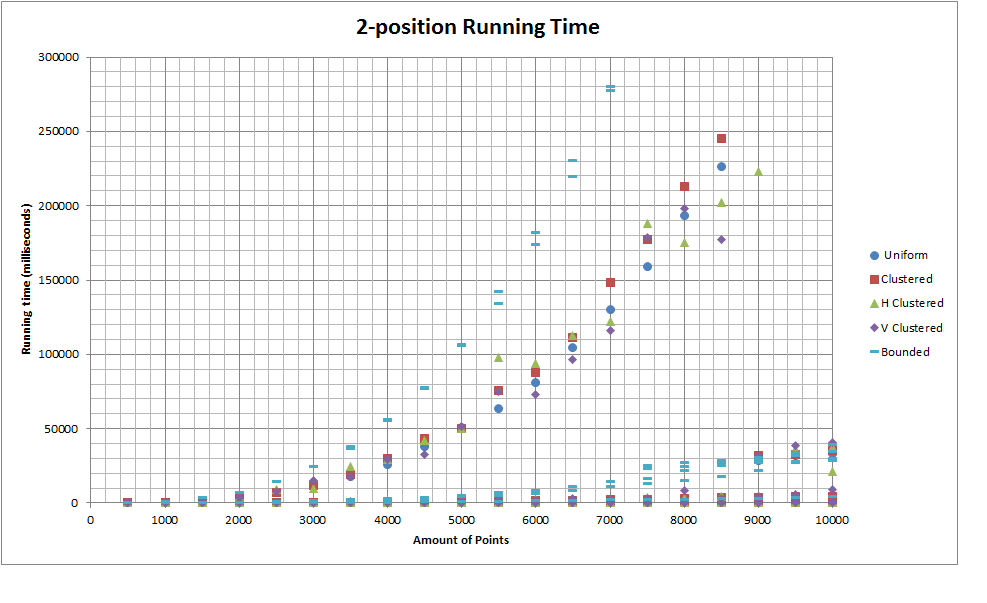
\includegraphics[scale = 0.5]{2PosRunningTime.png}}
  \caption{The running time of the 2-position algorithm}
 \end{figure}

\begin{figure}[H]
 \centering
  \centerline{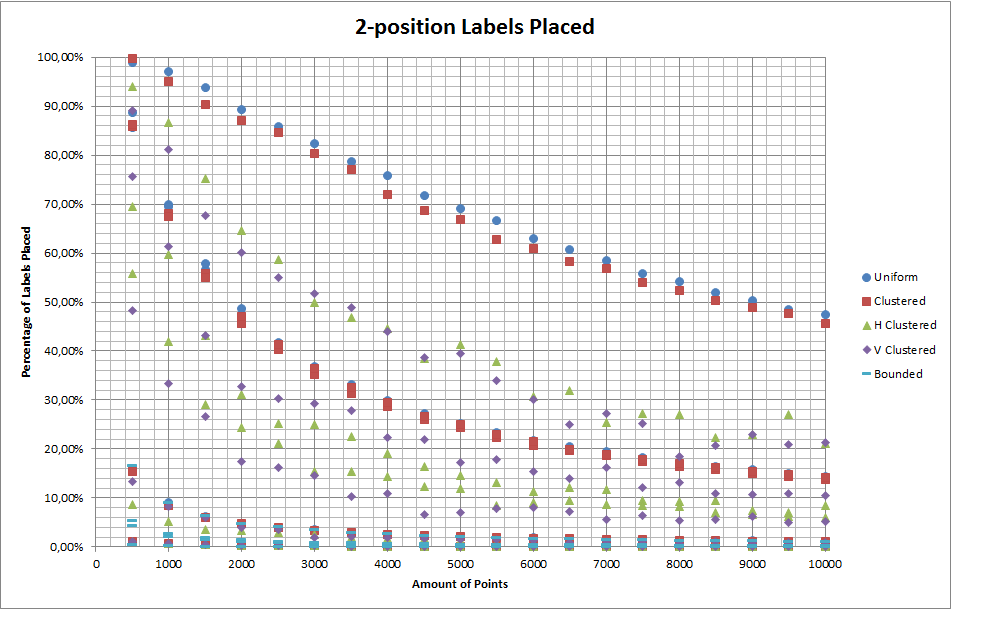
\includegraphics[scale = 0.5]{2PosLabelsPlaced.png}}
  \caption{The percentage of labels placed by the 2-position algorithm}
 \end{figure}

\subsubsection{Discussion}
As stated in section 2.2.1 the theoretical running time of the 2-position algorithm is $O(n^2)$. From figure 2 we can see that the running time of most of the cases are quite low. They take less than 10000 milliseconds to place all the labels. This is because the amount of collisions that the candidates have is small, so it will not take much time to map the collisions and it will take less time to place the labels. There are some cases that have higher running time than the others. We can see from the figure that the practical worst case running times are close to the theoretical running time $O(n^2)$. The running time in practice thus seems to be $\Omega(nlogn)$ best case and $O(n^2)$ worst case.\\
The worst cases, label size of 5000 by 5000, of each distribution suddenly drop when 7000 points is reached for bounded and 8500 points for the other distributions. This is because in these cases, there are many collisions. If we were to use the regular algorithm, the running time would exceed 5 minutes. So in that case, we use a greedy algorithm to place the labels, which takes much less time.\\
Other than the running time, we also look at the amount of labels our algorithm placed. As we can see from figure 3, when the amount of points is small, the algorithm gives solutions with a high percentage of placed labels. For uniform cases and clustered cases, our algorithm gives a high solution, and for most of the cases except for bounded cases. When the amount of points become higher, the percentage of placed labels will become lower. This is expected as the distribution and area stays the same but the amount of points increases. Uniform cases and clustered cases have more labels than the others in most cases. The reason why bounded cases have few labels is because all points are placed in a small area, this causes more overlaps for the candidates.\\
Compared to the 4-position and 1-slider algorithms the 2-position algorithm places the lowest percentage of labels. The running time is however smaller than that of the 4-position and 1-slider algorithms. 


\subsection{4-position}
\subsubsection{Results}
The algorithm of the 4-position model is explained in full detail in section 2.2. It is similar to the algorithm for the 2-position model, except it has two more candidates per point. A visual explanation of the 4-position model can be seen in figure 1.\\
 For the experimental evaluation of the 4-position algorithm we also used $2500$ different test cases with $500$ cases for each distribution. The running times of the test cases can be found in figure 4 and the percentage of points the algorithm could label can be found in figure 5.\\

 \begin{figure}[H]
 \centering
 \centerline{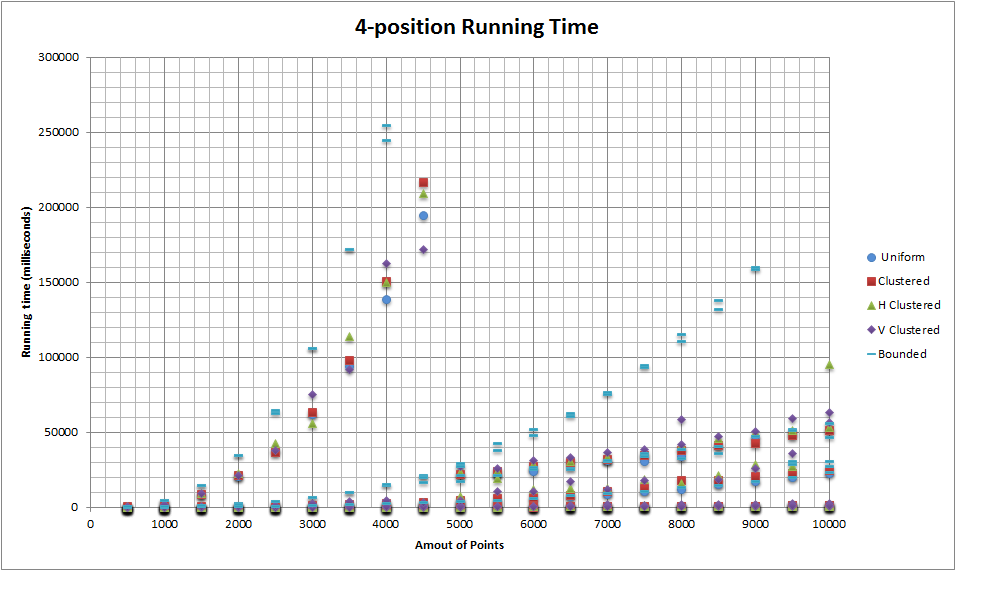
\includegraphics[scale = 0.5]{4PosRunningTime.png}}
 \caption{The Running Time of the 4-position algorithm}
 \end{figure}

 \begin{figure}[H]
 \centering
  \centerline{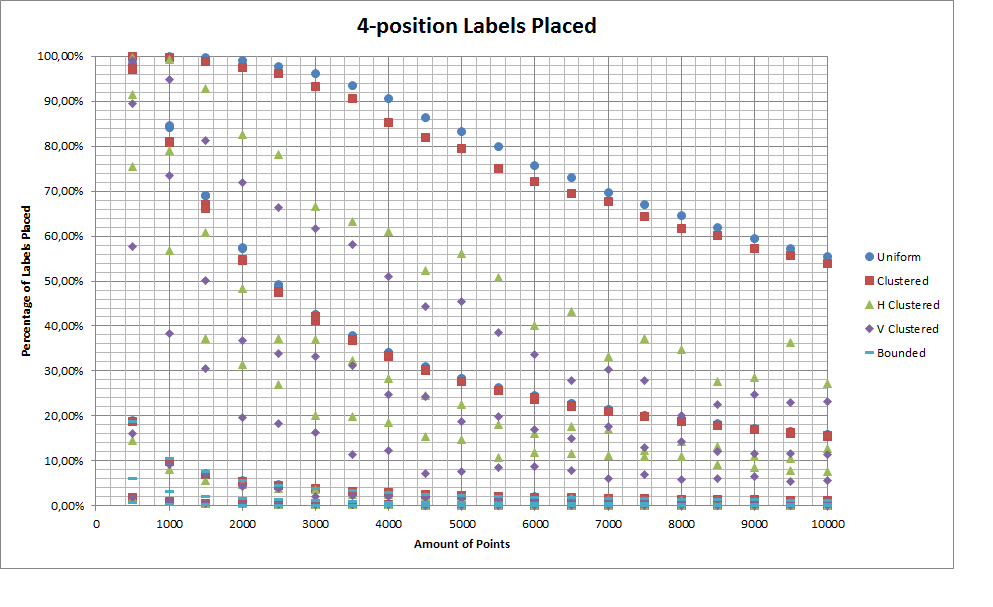
\includegraphics[scale = 0.5]{4PosLabelsPlaced.png}}
  \caption{The percentage of labels placed by the 4-position algorithm}
 \end{figure}

\subsubsection{Discussion}
As we stated in earlier, the algorithm for the 4-position model is nearly the same as the algorithm for the 2-position model. Hence the theoretical running time of the 4-position algorithm is also $O(n^2)$. In figure 4, it shows the running time for all $2500$ different cases. As with the algorithm for the 2-position model, the running time for most of the cases is close to $O(n\log n)$. This is because in most cases the amount of collisions is not $\Theta(n^2)$, so it will not take $\Theta(n^2)$ to map the collisions and it will also take less time to place the labels. We can see from the figure that the practical worst-case running time is close to the theoretical running time $O(n^2)$. The running time in practice thus seems to be $\Theta(n \log n)$ best case and $O(n^2)$ worst case.\\
Just as with the 2-position model, the highest running times of each distribution also suddenly drop when 3500 points is reached. This is because, in these cases, there are too many collisions and, as with the 2-position algorithm, we use a greedy algorithm to place the labels. However, there are still some differences between the algorithm for the 2-position model and the 4-position model. The 4-position algorithm reverts to using the greedy algorithm faster than 2-position algorithm. This is because, with the 4-position model, more collisions occur between candidates as there are more candidates in total.\\
Other than running time, we also look at the amount of placed labels of our algorithm. As we can see from figure 5, when the amount of points is small, the algorithm gives solutions with a high percentage of placed labels. When the amount of points become higher, the percentage of placed labels will become lower. This can be explained by the same situation in 2-position model. Uniform cases and clustered cases have higher percentage of placed labels than the other distributions in most cases and the bounded cases can place a low percentage of labels.\\
Compared to the 2-position and 1-slider algorithms the 4-position algorithm manages to place the highest percentage of labels. It has a worse running time compared to the 2-position algorithm but is quicker than the 1-slider algorithm.\\


\subsection{1-slider}
\subsubsection{Results}
For the evaluation of the 1-slider algorithm we ran 500 test cases (in contrary to the 2500 for the other placement models), 100 for each distribution. These test cases start with 500 points and increase by 500 points until it reaches 10000 points. We chose to have fewer test cases since our algorithm for the 1-slider tends to approach 5 minutes and it would else take days to run all 2500 testcases. The 1-slider algorithm is explained in full detail in section 2.3. An example of the 1-slider model can be found in figure 1.\\
 The running times of the test cases can be found in figure 6 and the percentage of points the algorithm could label can be found in figure 7.

 \begin{figure}[H]
 \centering
 \centerline{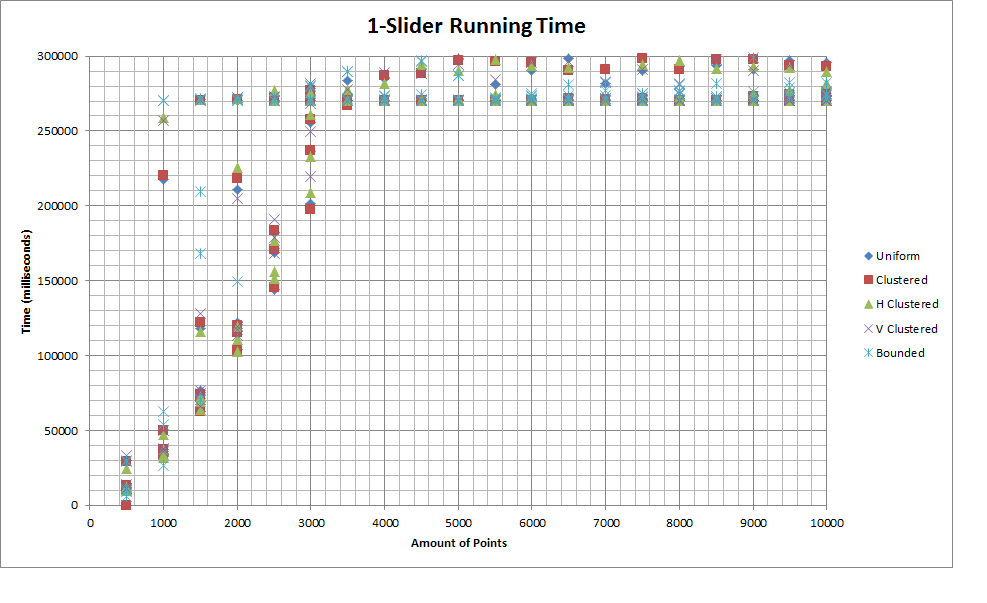
\includegraphics[scale = 0.65]{1slider.png}}
 \caption{The running time of the 1-slider algorithm}
 \end{figure}

 \begin{figure}[H]
 \centering
  \centerline{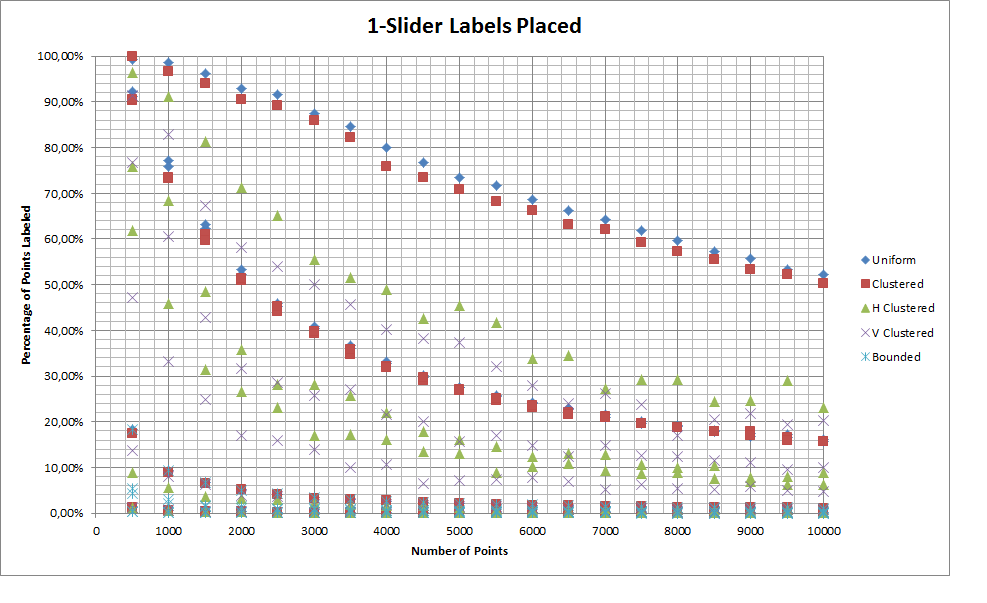
\includegraphics[scale = 0.65]{1sliderplaced.png}}
  \caption{The percentage of labels placed by the 1-slider algorithm}
 \end{figure}

\subsubsection{Discussion}
From section 2.3.9 we find that the theoretical running time of the 1-slider algorithm is $O(n^3)$. From figure 6 we can see that the practical running time of the 500 test cases matches the theoretical running time. The figure also shows that the running time of all the test cases plateaus after 3000 points is reached. This is because after 4.5 minutes has been reached we stop the algorithm and report the best solution found until then. From testing we found that ending the algorithm after 4.5 minutes left enough time for the algorithm to terminate and return the solution it had found such that it did not run longer than 5 minutes.\\
In figure 7 we can see the percentage of points that have been assigned a label. As usual, the amount of points that could be labelled decreases as the amount of points increases with the bounded test cases being affected the most.
 When we compare the results to the 2-position algorithm in figure 3, we see that the 1-slider manages to place slightly more labels. However, when we compare the results of the 1-slider to the results of the 4-position in figure 5, we can see that it manages to place considerably less labels. The 1-slider algorithm has a worse running time compared to both the 2-position algorithm and the 4-position algorithm.

\end{document}
